\section*{Robot SARA Hardware Description}

\setlength\intextsep{0pt}
\begin{wrapfigure}[10]{r}{0.3\textwidth}
	\centering
	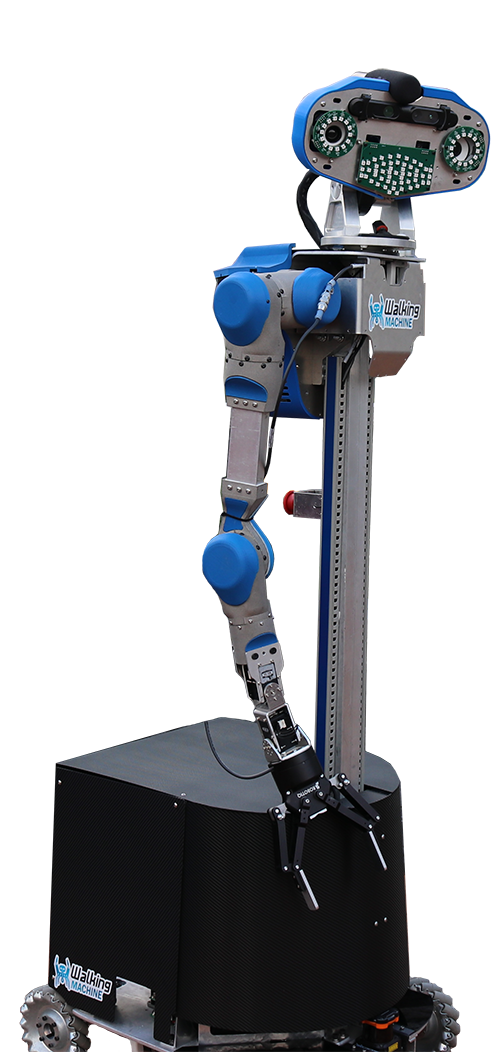
\includegraphics[width=0.25\textwidth]{images/sara.png}
	\caption{Robot SARA}
	\label{fig:wall-e}
\end{wrapfigure}

Specifications for robot SARA are as follows:

\begin{itemize}
	\item Base: Custom base with fully holonomic Mecanum wheel platform.
	\item Torso: 1 vertical DoF (future implementation).
	\item Right arm: Mounted on torso. 5-DoF custom arm made of Kinova motors.
	\item Neck: Tilt unit using one Dynamixel MX-64R servo actuator.
	\item Head: Custom head made of RGB neopixels leds and Asus Xtion Pro.
	\item Gripper: Robotiq hand 2 fingers 85mm.
	\item Robot dimensions: Base : 0,61m X 0,77m Height : 1,68m.
	\item Robot weight: 100kg.
	\item Additional sensors: Hokuyo UTM-30LX on base.
	\item Microphone: Rode microphone
	\item Batteries: 1x 24V 8 cells Lithium-ion battery
	\item Computer: 1x Lenovo p50 with 32GB RAM and nVidia Quadro M2000 4GB, 1x BeagleBone Black
	
\end{itemize}


\section*{Robot's Software Description}


For our robot we are using the following software:

\begin{itemize}
	\item Platform: Robotic Operating System (ROS) Indigo
	\item Navigation, localization and mapping: RTAB-Map, Gmapping, AMCL, DWA
	\item Face recognition: Cob people detection
	\item Speech recognition: Pocketsphinx
	\item Speech generation: Espeak
	\item Object recognition: Object recognition kitchen
	\item Arms control: Moveit and Kinova API
	\item Task executors: SMACH
\end{itemize}